The underlying mechanism which causes timing noise is not understood. From its
first observation multiple models have been proposed which are able to describe
some of the features. However, the variety of ways timing noise manifests and
the uncertainty in the mechanisms at work have made it difficult for any
conclusive statements to be made about the models. Any timing noise model must
simultaneously explain the observed variations while also remaining consistent
with the models proposed to explain the other timing variation - glitches.  In
addition the timescale over which some features occur is similar or possibly
longer than the history of pulsar astronomy~$\sim 50$~years: this means the
data is `incomplete' making conclusive statements impossible. Observations of
new features prompt new models for timing noise; as a result the timing noise
interpretations have evolved with the observations. We will present an overview
of both in this section.

\subsection{Random walk models}
\label{sec: TN interpretations random walk models}

Timing noise was first quantified and interpreted by \citet{Boynton1972} as a
Poisson like random walk in one of the phase, frequency, or spindown. The
pulsar spins down according to the power law spindown of equation \eqref{eqn:
power law spindown} except that at random times the pulse phase, frequency or
spindown jumps, or changes discontinuously. The waiting times between events
are Poisson distributed with a rate R such that over a period $T$ the number of
events follows a Poisson distribution with mean RT. All the jumps are
independent and the magnitudes are randomly distributed with means given by
$\langle\dP\rangle$, $\langle\dF\rangle$, and $\langle\dS\rangle$ for the phase
frequency and spindown. We can investigate the statistical properties of such
random walks by splitting the phase into contributions from the secular
spindown $\phi_{\mathrm{S}}$ (as given by equation \eqref{eqn: Taylor compact})
and contributions from the random walks
\begin{equation}
    \phi = \phi_{\mathrm{S}} + \Delta\phi_{\mathrm{R}}
\end{equation}
The three random walks can be written as the sum of $N$ individual events
occurring at times $t_{i}$
\begin{align}
    \Delta\phi_{\mathrm{R}} & = \s{i=1}{N}\Delta\phi_{i} H(t - t_{i}) 
     && \mathrm{(phase),} \\
    \Delta\phi_{\mathrm{R}} & = \s{i=1}{N}\Delta\f_{i} (t-t_{i})H(t - t_{i}) 
     && \mathrm{(frequency),} \\
    \Delta\phi_{\mathrm{R}} & = \s{i=1}{N}\frac{1}{2}\Delta\fdot_{i} (t-t_{i})^{2}H(t - t_{i}) 
     && \mathrm{(spindown),}
\end{align}
where $H(t)$ is unit step function at $t=0$. It should be noted that here we are
treating the three types of noise separately such that timing noise residuals 
from either a random walk in phase, frequency, or spindown; work by \citet{Cordes1980}
extended this model to handle mixing between the types of noise.

Timing noise is the remainder having
fitted and subtracted a second order Taylor expansion. Provided the perturbations
of $\phi_{\mathrm{s}}$ are small then the remainder will be exactly given by 
$\phi_{\mathrm{s}}$. Then, as described by \citet{Boynton1972} we can then 
average over: the $\dP_{i}, \dF_{i}$ or $\dS_{i}$
distributions, the $t_{i}$ distribution, and the $N$ distributions to give
\begin{align}
    \langle \Delta\phi_{R} \rangle & = \langle \dP \rangle R T 
    = S_{\mathrm{PN}}T && \mathrm{(phase),} \\
    \langle \Delta\phi_{R} \rangle & = \frac{1}{2}\langle \dF \rangle R T^{2} 
    = \frac{1}{2}S_{\mathrm{FN}}T^{2} && \mathrm{(frequency),} \\
    \langle \Delta\phi_{R} \rangle & = \frac{1}{6}\langle \dS \rangle R T^{3} 
    = \frac{1}{6}S_{\mathrm{SN}}T^{3} && \mathrm{(spindown).} \\
\end{align}
Here we have implicitly defined the strength parameters which combine the rate 
and averaged magnitude of jumps into a single quantity. Measurements of timing 
noise, if they are discreet events, will observe the accumulation of many 
individual events. As a result only the strength can be
measured, not the rate and average magnitude.

The three types of noise are distinguishable by their dependence on the
observation time $T$. The type of noise can be measured by
translating this into the dispersion measure of
$\Delta\fddot$ after fitting a cubic, or by inspection of the power spectrum.
\citet{Boynton1972} was able to categorise the Crab pulsar as frequency like noise.
They found that over a $5$~year period the noise process was stationary
and consistent with the frequency noise hypothesis. No deterministic process
could account for the timing residuals strengthening their conviction that some
random process was taking place.  However, they suggested that over longer periods
the random walk will be non-stationary due to either mixing with other types of
walks, or decay of the strength parameter with time.

The interpretation of timing noise as a Poisson random walk is a purely
statistical model. It is however backed up for a rich variety of physical
models.  A key feature of any physical
random walk model is that it must be able to produce both increases and
decreases in the relevant parameter. For this reason it is felt unlikely that
the timing noise mechanism is the same as the glitch mechanism, although they
must be related.  In addition it is unclear if timing noise is a continuous or
discreet process, certainly if it is discreet the waiting time between events
must be shorter than the shortest observation periods $\sim days$. 

The first physical model was proposed by \citet{Boynton1972}, the noise process
consisted of the as accretion of small lumps of matter onto the NS from the
interstellar medium. Lumps of matter fall randomly onto the surface of the star
causing either a spin-up or slowdown through the transfer of angular momentum.
After this many models were proposed such as starquakes and the random pinning
and unpinning of vortex lines; these were reviewed by \citet{Cordes1981} and
evaluated against observational constraints. Of these only three mechanisms
where found to be consistent with observations: crust breaking by vortex pinning, a
response to heat pulses, and luminosity related torque fluctuations. Since this
review, new random walk mechanisms have been proposed such as: variations in
the magnetospheric gap size \citep{Cheng1987}; the interference by debris entering
the magnetosphere \citep{Cordes2008}; and the accumulation of multiple micro-glitches
\citep{Janssen2006}. It would be a useful exercise to review both the new and 
old mechanisms against the current observational catalogue.

The first measurement of individual events was made by \citet{Cordes1985} who
identified $\sim20$ events in both frequency and spindown which could not be
explained by a glitch. In the same work, considering 24 pulsars over a period
of~$\sim13$~years, the authors concluded that: the timing noise seen in the
data could not be explained solely by an idealised random walk processes in the
phase, or its derivatives. They suggested that most of the activity is due to a
mixture of events in the phase, frequency and/or frequency derivative.

A recent review, and the most comprehensive by far was performed by
\citet{Hobbs2010} for 366 pulsars. They found that, timing residuals tend to
admit quasi-periodic features when observed on sufficiently long time scales
$\gtrsim 2$~years. As such, the method of measuring the type and strength of
timing noise depends on the length and epoch of observation. This suggests a
pure random walk hypothesis is not entirely consistent with observations.
Nevertheless, it is unclear what repercussions the conclusions of
\citet{Hobbs2010} has for the physical origin of timing noise.

\subsection{Free precession}
\label{sec: free precession}

A mechanism which could quite naturally produce strictly periodic variations in the
observable features of a pulsar is \emph{free precession}. This occurs in any
non-spherical body for which the angular momentum is not aligned with a principle
axis of the moment of inertia. Such a circumstance could arise given the
chaotic birth of NSs. However, we must be clear that the timing noise induced by 
precession alone would be strictly deterministic; this is something which we do
not observe.
It is instructive however to consider the mechanics of precession since it will
be visited later on.

In the simplest case imagine an biaxial body, 
rotating about an axis $\Omega$. with a moment of inertia given by 
\begin{equation}
    I = \left[\begin{array}{ccc}
            I_{0} & 0 & 0 \\
            0 & I_{0} & 0 \\
            0 & 0 & I_{0}(1 + \epsilon)
            \end{array}\right],
\end{equation}
where $\epsilon \ll 1$ is the measure of oblateness or prolateness.  If the
body is free from torques, then in the rotating frame of the body, Euler's
equations of motion (see section \ref{sec: neutron star dynamics in the
rotating frame}) are given by
\begin{equation}
    I\dot{\bm{\Omega}} + \bm{\Omega} \times \left(I\bm{\Omega}\right)=0.
\end{equation}
This is a system of three coupled ODEs. Writing the components of the spin
vector as $\bm{\Omega} = [\Omega_{x}, \Omega_{y}, \Omega{z}]$, we have the
set of equations:
\begin{align}
\dot{\Omega}_x = -\Omega_y\Omega_z, &&
\dot{\Omega}_y = \Omega_x \Omega_z, &&
\dot{\Omega}_z = 0
\end{align}
We can find a solution by first realising that $\Omega_{z}=\mathrm{const}$.
We are then left with a set of
two coupled ODEs, solving these with appropriate intial conditions 
the solutions take the form
\begin{align}
    \Omega_{x} & = \Omega_{0}\sin(a_0)\sin\left(\Omega_{0}\cos(a_0)\epsilon t\right), \\
    \Omega_{y} & = \Omega_{0}\sin(a_0)\cos\left(\Omega_{0}\cos(a_0)\epsilon t\right),\\
    \Omega_{z} & = \Omega_0 \cos(a_0),
\end{align}
where $a_0$ is the angle between the spin-vector and the body frame $z$ axis and
$\Omega_0$ is the magnitude of the spin-vector. 

We observe that the spin axis of the body will trace out a cone about the $z$
principle axis of the moment of inertia with a period of
$\frac{1}{\Omega_{z}\epsilon}$.  The half-angle of the cone is set by the
initial conditions and will not evolve. This is the motion of free precession
and is illustrated in figure \ref{fig: precession}. 
\begin{figure}[htb]
\centering
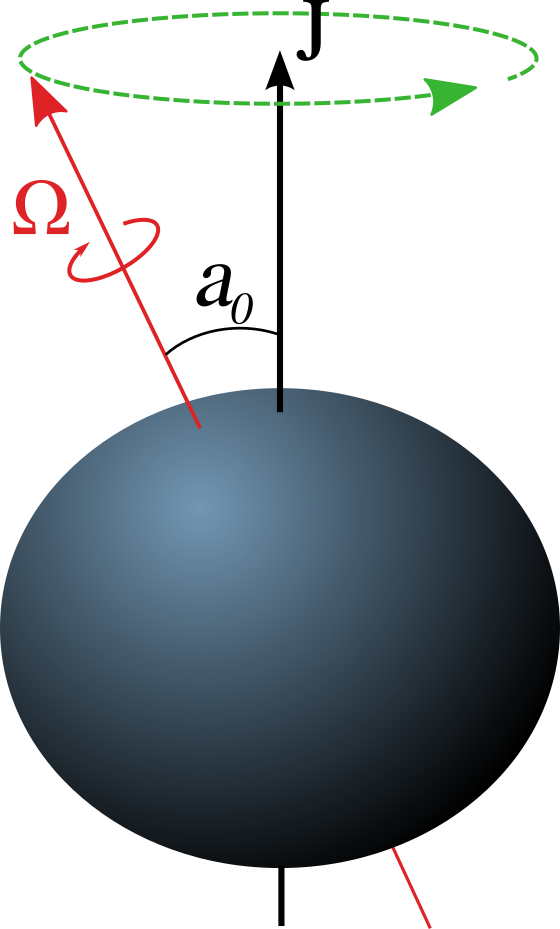
\includegraphics[scale=0.2]{Precession.png}
\caption{Illustration of free precession for a simple biaxial body. The spin
    axis $\spin$ traces out a cone about the angular momentum vector $\mathbf{J}$.}
\label{fig: precession}
\end{figure}•

Neutron stars are assume to have a rigid crust, as such they may be non-axially
symmetric. Precession as a candidate to explain timing noise fluctuations was
first discussed by \citet{Ruderman1970}. He found that the free precession
period was, for reasonable values of the  ellipticity $\epsilon$, able to
explain periodic fluctuations in the Crab pulsar. Of the known Neutron star 
physics, one of the few mechanism that could operate over the time-scales observed
in timing residuals is free precession. 

The favoured interpretation for glitches poses a problem for sustained free
precession as an interpretation of timing noise. Theoretical models suggest the
interior of a neutron star is a superfluid; most of the moment of inertia is
contained in an array of vortices which are pinned to the crust.  Glitch events
correspond to the sudden unpinning of these vortices. It was shown by
\citet{Shaham1977} that for perfect pinning the free precession frequency and
geometry were modified resulting in no slowly oscillating long-lived modes. In
the case of imperfect pinning \citet{Sedrakian1999} found that long-lived modes
existed but where damped.

Despite the inconsistency with the superfluid pinning model for glitches,
evidence was presented by \citet{Stairs2000} of free precession in pulsar
B1828-11. They found the phase residuals and variations in the pulse profile
could be accounted for by precession.  This was followed up by detailed
modelling of the effects by \citet{Akgun2006}.

Including the spindown from an applied torque \citet{Cordes1993} noted that
free precession may be driven by fluctuations that counter the damping process;
in turn, the precession can drive torque fluctuations. The effect is most
noticeable in young pulsars. 

Work by \citet{Jones2001} compared a model of free precession against the handful
of proposed observations of free precession. Their model included the feedback
between the torque and precession and required only the crust to undergo precession.
In all but one case such a model was found to be consistent with the observations.


\subsection{Two state switching}
\label{sec: two state switching}

Recently a new model has been proposed by \citet{Lyne2010} to explain the
observation that, over long time periods, the timing noise structure is
quasi-periodic. This began with the observation by \citet{Kramer2006} that the
pulses from PSR B1931+24 where intermittent. The pulsar acts as a normal pulsar
for $\sim10$~days and then switches off, being undetectable for $\sim25$~days,
and then switching on again. Analysing the spindown rate between the on and off
states, they determined the spindown rate $\dot{\f}$ was $\sim50\%$ faster in
the on state. This figure illustrating this is reproduced in figure \ref{fig:
kramer 2006 fig2}.
\begin{figure}
    \centering
    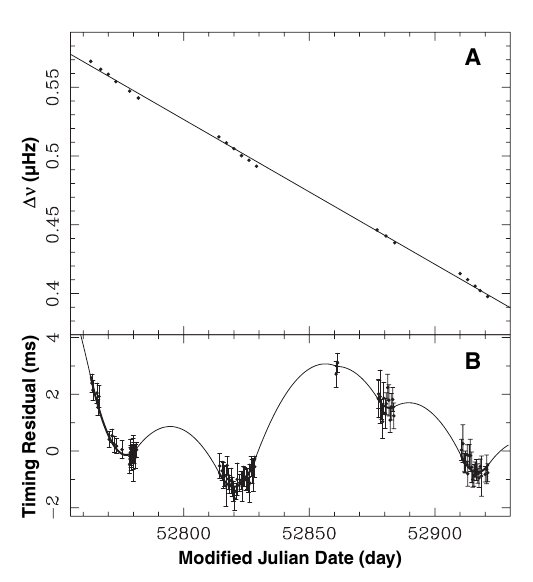
\includegraphics[width=.5\textwidth]{Kramer_2006_fig2}
    \caption{Figure taken from \citet{Kramer2006} showing the switched spindown
             of pulsar PSR B1931+24}
    \label{fig: kramer 2006 fig2}
\end{figure}
In the  upper panel (\textbf{A}) the authors show the evolution of the
rotational frequency over a 160 day period encompassing several switching
events. The line shows the long-term spindown of the pulsar while the dots show
individual measurements made during the on state. During these on states the
gradient of the reduction in frequency is increased, that is the spindown has
increased. It is thought that measurements of the frequency in the off state
would produce a line with decreased spindown connecting the dots. This is
accompanied by the timing residual measured over the same period in the lower
panel (\textbf{B}). This shows significant quasi-periodic modulations in sync
with the switching. This work proposed that the switching was a magnetospheric
phenomenon. The sharpness of the switches certainly requires something acting
on a short timescale and it intuitively makes sense that the greater spindown
results from greater torque produced by the emissions observed during the on
state.

The authors of \citet{Lyne2010} then tested a range of other pulsars and
presented a study of 17 pulsars for which they claim evidence for two-state
switching. Unlike B1931+24 these pulsars are not intermittent but 
continuously pulse. Measuring the spindown as a function of time over a
$\sim20$~year period they demonstrated fluctuations as reproduced in figure
\ref{fig: lyne 2010 fig2}

\begin{figure}
    \centering
    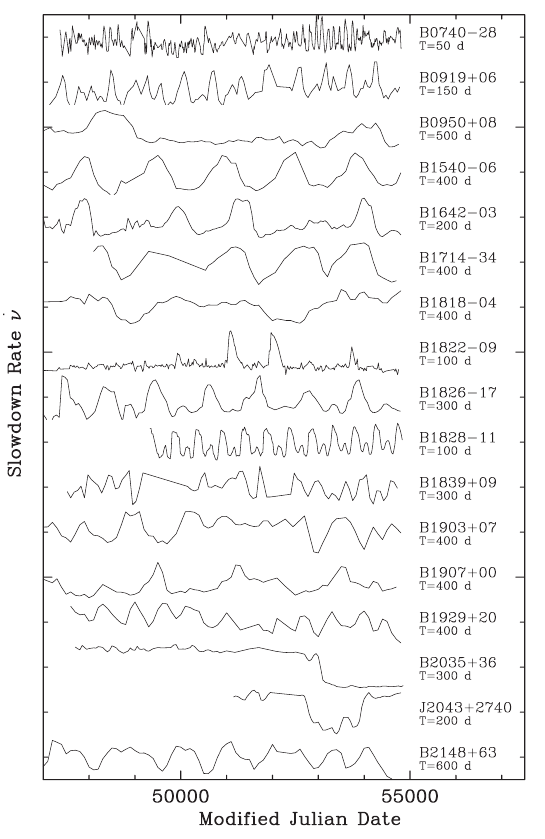
\includegraphics[width=.5\textwidth]{Lyne_2010_fig2}
    \caption{Figure taken from \citet{Lyne2010} showing the spindown rate
             of 17 pulsars over a $\sim20$~year period.}
    \label{fig: lyne 2010 fig2}
\end{figure}

This plot shows smooth variations in the spindown with some pulsars better
behaved than others. The method used to calculate the spindown required
averaging over a $\sim100$~day period; the authors argue that, if the spindown
undergoes a sharp switch between two values, this will be smoothed out by the
averaging.  Therefore it is argued in \citet{Lyne2010} that figure \ref{fig:
lyne 2010 fig2} show the $\dot{nu}$ moving between a few (typically 2) well
defined values.  The authors noted a gradual long-term change in the spindown
for all pulsars across the data set, indicating a non-zero second order
spindown. 

In order to quantify the claim of \citet{Kramer2006} that the switching was
magnetospheric (e.g. the results of enhanced particle flow), \citet{Lyne2010}
looked for correlations between the pulse width, measuring the amount of
emission, with the spindown rate.  They found that for 6 pulsars the pulse
width was indeed wider during the higher spindown. However, these variations
are also smooth and subject to the same averaging process. To improve the
resolution they then show the individual measurements of pulse width for two of
the pulsars; these appear to demonstrate the switching happening
instantaneously between the two values. The authors argue this confirms that
the two-state switching is magnetospheric since this is the only mechanism able
to act on such short timescales. Intuitively it makes sense that changes in
the pulse shape, will be correlated with changed in the amount of emission and 
hence the spindown rate. 

It has not been established how these magnetospheric will manifest themselves.
In particular this interpretation lacks an explanation of how the magnetosphere is
regulated to stay in a stable state for long periods ($1-10$~years) but then
switch over $\lesssim100$~days.

\citet{Lyne2010} proposes that the quasi-periodic structure observed in many
timing residuals (e.g. see \citet{Hobbs2010}) could be explain by this
switching process. To quantify this, in the supplementary material they created
a simple model for the effect of switching in the value of the spindown
$\dot{\nu}$ on timing residuals. We will now repeat this experiment to outline
the results. 

Firstly we model a pulsar as spinning down in the usual way except that it's
spindown has two distinct values $\dot{\nu}_{A}$ and $\dot{\nu}_{B}$. Then we
define the model the ratio of time spent state in state $A$ and $B$ as $R =
t_{B}/t_{A}$.  This is a purely deterministic model and having generated the
spindown values we can integrated twice to get the phase. Fitting and
subtracting a quadratic polynomial leaves the phase residual. In figure
\ref{fig: lyne example D=0} we show a typical result; in the top figure is the
spindown values which we define and in the bottom the resulting structure in
the phase residual.
\begin{figure}[htb]
    \centering
    \includegraphics[width=.5\textwidth]{{R_3.0_D_0}.pdf}
    \caption{A deterministic realisation of the Lyne switched spindown model. The
             resulting structure in the timing residuals are strictly periodic.}
    \label{fig: lyne example D=0}
\end{figure}
The phase residuals in figure \ref{fig: lyne example D=0} are strictly
periodic. \citet{Lyne2010} realised that in order to fit the observed
quasi-periodic residuals a random element must be introduced. This can be done
by the form of a 'dither' $D$ in the waiting time between switches. Now we have
periods $t_{A}^{i}$ and $t_{B}^{i}$ which are Gaussian distributed with a mean
of $t_{A}$ and $t_{B}$ and a standard deviation $D t_{A}$ and $D t_{B}$. The
result is illustrated in figure \ref{fig: lyne example D=0.3}.

\begin{figure}[htb]
    \centering
    \includegraphics[width=.5\textwidth]{{R_3.0_D_0.3}.pdf}
    \caption{A realisation of the Lyne model with a random element producing the
             observed quasi-period structure.}
    \label{fig: lyne example D=0.3}
\end{figure}


\citet{Lyne2010} argue that the fast state changes seem to rule out free
precession as the origin of oscillatory behaviour observed in timing residuals.
One of the pulsars which shows some evidence for two state switching is PSR
B1828-11; this pulsar was cited as evidence for free precession by
\citet{Akgun2006}. \citet{Lyne2010} argue that the fluctuations from this pulsar
should be reinterpreted as two-state switch due to the observed fast state
changes. 

\citet{Jones2012} argues that such dismissal of precession is premature
since the modulation period of the switching has yet to be explained.  Instead,
the idea is raised that precession and magnetospheric switching are not
mutually exclusive.  Pulsars are most probably born in a randomly distributed
magnetospheric state, at least some may therefore exist under a delicate
balance between two states. Precession may be capable of periodically varying
the statistical probability of existing in one state or the other, sharp
changes would be caused by an `avalanche effect' as the particle energies reach
a threshold.  This provides the timescale for switching along with the ability
for the switching to be quasi-periodic since the precession only biases the
probability.

A similar idea considered by \citet{Cordes2013} interpreted two state switching
as evidence for a system in a state of stochastic resonance.  This occurs in
systems in which, under certain conditions, a weak periodic forcing function is
amplified by stochastic noise.  To explain this phenomenon in appendix
\ref{App: Stochastic} we present a toy model of stochastic resonance for a
particle in a well. The switching could therefore be the result of any periodic
modulation, such as precession, coupled to random fluctuations. This would quite
naturally explain the stability of states, the timescales over which the occur,
and the fact that it is observed in only some pulsars.

\subsection{Evidence from anomalous braking indices}
\label{sec: evidence from anomalous braking indices}

An alternative motivation to study timing noise comes from the measurement of
anomalous braking indices. The pulsar braking index is defined by $n$ in
equation \ref{eqn: power law spindown}.  Rearranging this equation as in
\eqref{eqn: measured braking index} the braking index can be measured for
observed pulsars. Different types of braking exhibit different braking indices.
It is therefore a reasonable idea to measure the braking index and calculate
the type of braking. Pulsars spun down by an electromagnetic torque should
follow a braking index of $n=3$, while gravitational wave spindown has $n=5$.

Measuring these indices for the known pulsar population we do not find a consensus
on the type of braking. Values from from unity up to $10^{6}$ and even negative
braking indices have been measured. These are known as \emph{anomalous}
braking indices. 

Recent work by \citet{Biryukov2012} observed that
younger pulsars tend to have braking indices of the correct order of
magnitude. However, beyond~$\tau_{ch}\approx10^{5}$~years
the absolute value of the braking index rapidly grows,
reaching values as large as $10^{6}$ for the oldest pulsar. In addition an
almost equal number of pulsars have positive and negative values of the braking
index. The figure demonstrating this is plotted in
figure~\ref{fig: braking indices}.

\begin{figure}[ht]
\centering
	\includegraphics[width=0.5\textwidth,trim=0mm -10mm 0mm 0mm]
               {{Biryukov_2012_Figure_7}.png}
\caption{Pulsar population in the $n_{obs}-\tau_{ch}$ diagram image from
\citet{Biryukov2012}}
\label{fig: braking indices}
\end{figure}

\citet{Biryukov2012} proposed that the spindown $\dot{\nu}(t)$ may contain the
secular spin down $\dot{\nu}_{\textrm{sec}}(t)$ and a cyclic component
$\dot{\nu}_{\textrm{sec}}(t)\epsilon(t)\nu(t)$ oscillating the spindown about
a mean value. Taking a simple case where the cyclic term has the form $A
\cos\phi(t)$ where $A$ is the relative amplitude of the oscillations and
$\phi(t)$ is linear in $t$, the authors derive an equation for the observed braking
index

\begin{equation}
n_{obs}(t) =
\frac{n}{1+A\cos(\dot{\phi}t+\phi_0)}
+\frac{(n-1)(kt-c)}{(1+A\cos(\dot{\phi}t+\phi_{0}))^{2}}A\dot{\phi}\sin(\dot{\phi}t+\phi_{0}).
\label{eqn: nobs}
\end{equation}•

This observed braking index contains a constant positive term oscillating about
the true braking index and a term which grows linearly in time. The authors found 
that for $\tau_{ch}<10^{5}$ yrs the linear term is negligible and so we observe
approximately the real braking index $n$. At later times the linear term
drives the observed braking index to larger values while a sinusoidal term produces
positive and negative values. In figure \ref{fig: nobs} we plot the trajectory
of a single pulsar following equation \eqref{eqn: nobs}. The authors claim each
of the pulsars in \ref{fig: braking indices} is following a similar trajectory.

\begin{figure}[ht]
\centering
	\includegraphics[width=0.5\textwidth]
               {{Analytic_Monotonic_and_Cyclic}.png}
\caption{A sketch of the observed braking index according to
equation \eqref{eqn: nobs}, the values here are intended for a qualitative
overview rather than analysis. }
\label{fig: nobs}
\end{figure} 

This simplistic idea is able to explain some of the defining features of the
known pulsar population braking indices. This requires a mechanism to modulate
the spindown over long timescales. By fitting their model to data, they
estimate the timescale to be of the order $10^{3}-10^{4}$~years. At least one
physical model, precession, could produce variations on the required timescale.
However, this is significantly longer than the precession timescales invoked to
explain the fluctuations in timing residuals which were $1-10$~years.
\begin{subappendices}
\subsection{Toy model of stochastic resonance: particle in a potential}
\label{App: Stochastic}

Here we present a simple toy model of stochastic resonance. This is a
statistical phenomena occurring when a weak periodic forcing function is
amplified by noise (see \citet{Jung1991} for a full treatment).  For the
application to neutron stars, see \citet{Cordes2013}; here we simply aim to
describe the essential features of stochastic resonance (not its application to
NSs). 

We will consider a particle at a position $x$ which is subject to some
potential and acted upon by a forcing function $F(t)$. In general though, $x$
could be any state variable, thus stochastic resonance could be produced
in many systems.

First consider the static case of a particle in a potential $U(x)$  given by:
\begin{equation}
    U(x) = \frac{x^{4}}{4}-\frac{x^{2}}{2}. 
\end{equation}
This potential is characterised by two wells at $\pm1$, a maximum exists
between them at the origin. The particle in one of the wells sees a potential
barrier $\Delta U$ corresponding to the height of the maximum above its
position.

Assume the particle is acted upon by a random forcing function $F(t)$ which is
modelled as a Gaussian white noise with strength $D$. Depending on the
magnitude of $D$ with respect to the potential, the motion of the particle
admits two distinct cases:
\begin{enumerate}
\item $D \ll \Delta U \;\;$ in which case the particle remains inside whichever
    well it initially starts in and does not escape.
\item $D \gg \Delta U \;\;$ in this case the particle will not see the the
    individual wells only the larger one.
\end{enumerate}

The motion of the particle obeys the following equation of motion:
\begin{equation}
    \frac{dx}{dt} = -\frac{\partial V(x,t)}{\partial x} + F(t). 
\end{equation}
The motion of the particle has two components, the deterministic effect of the
potential and random fluctuations.

We now modify the potential to be acted on by a weak periodic function; this
introduced a third possible type of behaviour. Writing the time dependant
potential as
\begin{equation}
    V(x,t) = \frac{x^{4}}{4}-\frac{x^{2}}{2} + \epsilon x \cos(\omega_{0} t).
\end{equation}
Inserting this potential into the equations of motion:
\begin{equation}
    \frac{dx}{dt} =  x - x^{3} + F(t) + \epsilon \cos(\omega_{0} t).
\label{eqn:stochastic eom}
\end{equation}
Solving this numerically we fix $\epsilon=0.001$,
$\omega_{0}=\frac{2\pi}{10}$ and choose three values of $D$ which illustrate
typical behaviours of the solution
\begin{figure}[ht]
\centering
   \includegraphics[width=0.4\textwidth,trim=0mm -10mm 0mm 0mm]
   {{Stochastic_resonance}.png}

\caption{Three solutions to equation \eqref{eqn:stochastic eom} changing the
    random forcing functions strength $D$. The first and last panels show the
    deterministic solutions for the particle position: either the forcing
    function is weak compared to the potential, the particle remains in well in
    which it begins; or the forcing function is much stronger than the
    potential and so the particle freely moves about the two wells. The middle
    panel illustrates the special case of stochastic resonance whereby the
periodic fluctuations of the potential allow quasi-periodic variations in the
particles position between the two wells.}

\label{fig:stochastic resonance}
\end{figure}
The first and last runs replicate the behaviour expected  for a static well,
either the particle is confined to the well it starts in, or the random noise
is too strong and the individual wells are not observed. The middle case
displays strong stochastic resonance: the solution
displays a switching between bi-stable states but does not strictly follow the
period of the forcing function. The
important point here is that the forcing function may be weak, but provided it
is periodic or at least quasi-periodic the signal is amplified by the random
noise such that it may be visible in data sets where it would typically be
considered lost.

\end{subappendices}
